\chapter{Radar FMCW}
\section*{Resumen}
En este capítulo se exponen los fundamentos teóricos y los principios operativos del radar de onda continua modulada en frecuencia (FMCW). A diferencia de las arquitecturas de pulso convencionales, la tecnología FMCW fundamenta su funcionamiento en la emisión ininterrumpida de una señal cuya frecuencia varía en forma lineal en el tiempo. Se presentan las ecuaciones fundamentales que gobiernan la señal de batido resultante entre la señal transmitida y la reflejada. Asimismo, se analiza el impacto que poseen el ancho de banda ($B$) y el período de barrido ($T$) sobre la resolución en espacio y velocidad.

\section{Reseña histórica}
RADAR es un acrónimo originado durante la Segunda Guerra Mundial que significa \textit{Radio Detection and Ranging} (detección y medición de distancia mediante radio). Un sistema de radar está compuesto por un transmisor y un receptor de radiofrecuencia. El transmisor emite ondas electromagnéticas que se propagan por el espacio; al incidir sobre un objetivo y regresar al receptor, se mide el tiempo transcurrido entre la emisión y la recepción de su eco, tal como se ilustra en la Figura~\ref{fig:fig1}. Dado que las ondas de radio se propagan en el aire aproximadamente a la velocidad de la luz, es posible determinar la distancia al objetivo mediante la medición de dicho retardo temporal \cite{Charvat2014}.

\begin{figure}[H]
    \centering
    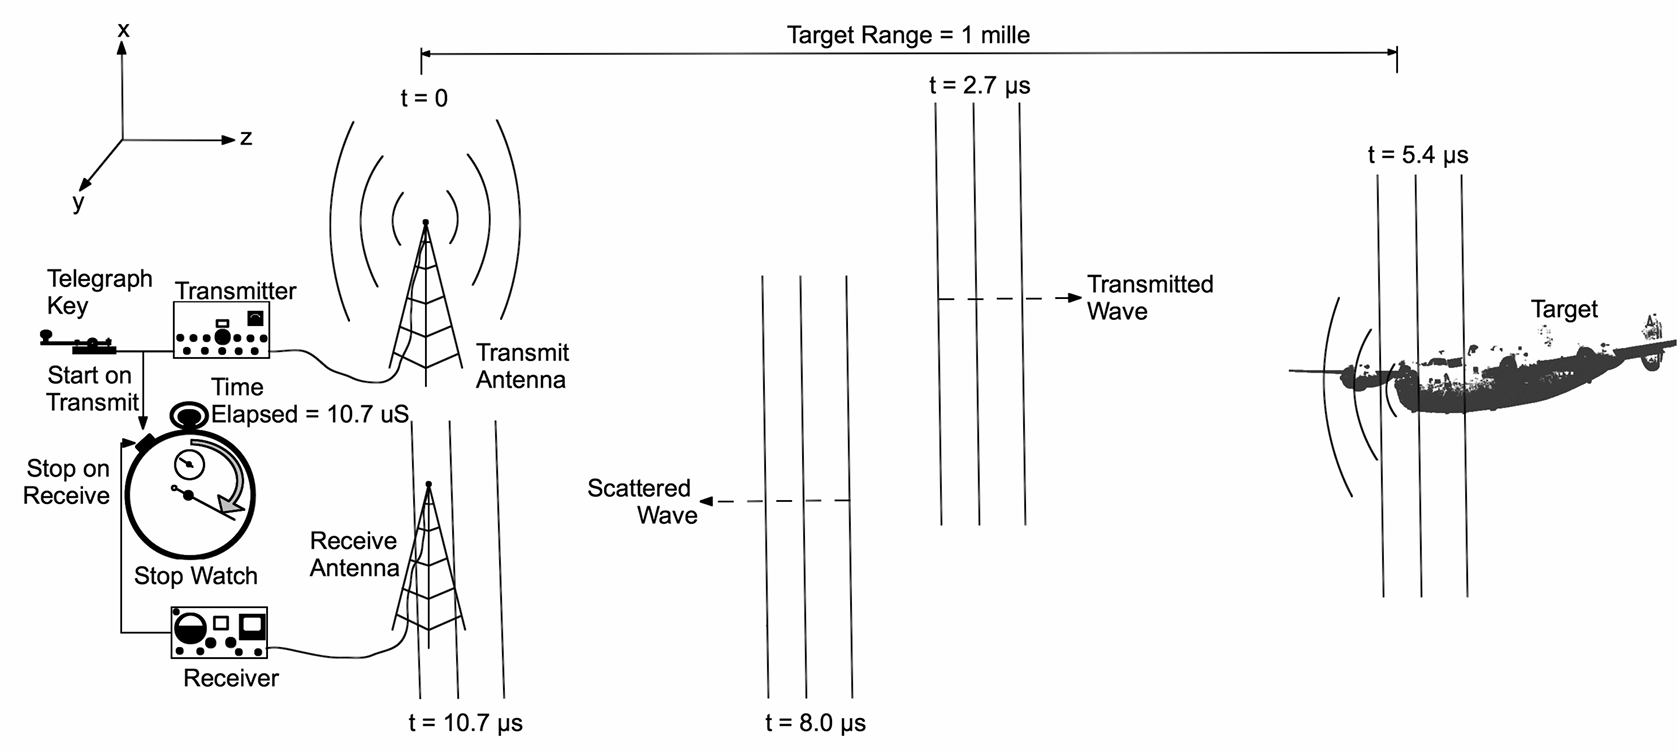
\includegraphics[width=0.75\linewidth]{imagenes/diagrama radar fmcw.png}
    \caption{Sistema de radar utilizado para la detección de un objetivo. (Fuente: \cite{Charvat2014}).}
    \label{fig:fig1}
\end{figure}

\section{Radar de onda continua modulada en frecuencia (FMCW)}

La incapacidad de un radar CW (onda continua) simple para medir la distancia a un objetivo está relacionada con el reducido ancho de banda de su señal transmitida. Para que sea posible determinar la distancia, es necesario incorporar algún tipo de referencia temporal que permita identificar el instante de transmisión y el instante de recepción de la señal reflejada. Cuanto más precisa sea esta referencia temporal, mayor será la exactitud en la medición del tiempo de propagación.

Una forma de incrementar el ancho de banda consiste en modular la portadora, ya sea en amplitud, frecuencia o fase. Una técnica ampliamente utilizada para ampliar el espectro de una señal de onda continua consiste en modular su frecuencia. En este caso, la información temporal está asociada a la variación de frecuencia de la señal transmitida. El tiempo de propagación puede determinarse a partir de la diferencia de frecuencia existente entre la señal transmitida y la señal reflejada recibida. Este principio constituye la base de funcionamiento de los radares de onda continua modulada en frecuencia (FMCW) \cite{Charvat2014}.

\subsection{Diagrama en bloques del radar FMCW}
El diagrama en bloques de este radar, presentado en la Figura~\ref{fig:fig2.4}, cuenta con los siguientes módulos:
\begin{itemize}
    \item \textbf{Generador de chirp:} Es el bloque en el que se centra la investigación de este documento. Se encarga de generar la onda continua modulada en frecuencia; en próximos capítulos se analizarán en detalle las secciones correspondientes.
    
    \item \textbf{ATT (Atenuador):} Ajusta el nivel de potencia de la señal del VCO antes de entrar al amplificador de potencia, evitando su saturación.
    
    \item \textbf{PA (Power Amplifier):} Amplifica la señal de RF hasta un nivel adecuado para su transmisión.

    \item \textbf{SPLTR (Divisor de señal):} Divide la señal del VCO en dos caminos: uno hacia la antena transmisora y otro hacia el mezclador (MXR) como oscilador local.

    \item \textbf{Antenas:} Una antena transmite la señal modulada y la otra recibe el eco reflejado por los objetos.

    \item \textbf{LNA (Low Noise Amplifier):} Amplifica la señal recibida con bajo nivel de ruido, preservando la relación señal/ruido.

    \item \textbf{MXR (Mezclador):} Mezcla la señal recibida (amplificada por el LNA) con la referencia del VCO. El resultado es la \textit{señal de batido}, cuya frecuencia es proporcional al retardo del eco y, por lo tanto, a la distancia.

    \item \textbf{SDR (Software Defined Radio):} Se encarga del procesamiento de la señal de batido.

    \item \textbf{Computadora:} Se utiliza para la programación de la SDR y la visualización de los resultados.
\end{itemize}

\begin{figure}[H]
    \centering
    
\includegraphics[width=0.75\linewidth]{imagenes/diagrama en bloques radar FMCW.png}
    \caption{Diagrama en bloques de un radar FMCW. (Fuente: Propia).}
    \label{fig:fig2.4}
\end{figure}

\subsection{Medición de distancia y velocidad Doppler}

En un radar de onda continua modulada en frecuencia (FMCW), la frecuencia transmitida varía con el tiempo de una manera conocida. Considerando el caso en que la frecuencia del transmisor aumenta linealmente con el tiempo, tal como se muestra en la Figura~\ref{fig:fig2.2}(a), si existe un objeto reflector situado a una distancia $R$, la señal reflejada regresará al radar luego de un tiempo:
\begin{equation}
    T = \frac{2R}{c}
\end{equation}
Donde $c$ es la velocidad de propagación de la onda electromagnética. Debido a este retardo temporal, la señal recibida constituye una versión retrasada de la señal transmitida. Si ambas señales se mezclan mediante un elemento no lineal, como un diodo o un mezclador, se genera una señal de frecuencia diferencia denominada frecuencia de batido $f_b$. En ausencia de movimiento relativo entre el radar y el objetivo, es decir, cuando no existe desplazamiento Doppler, la frecuencia de batido depende únicamente de la distancia al blanco. Si la frecuencia transmitida varía con una pendiente $f_0$ (expresada en Hz/s), la frecuencia de batido asociada al alcance resulta:
\begin{equation}
    f_r = f_0 T
\end{equation}
O, reemplazando el tiempo de retardo por su expresión en función de la distancia:
\begin{equation}
    f_r = \frac{2R}{c} f_0
\end{equation}
Por lo tanto, la frecuencia de batido es directamente proporcional a la distancia al objetivo. Midiendo esta frecuencia es posible determinar el alcance del blanco sin necesidad de transmitir pulsos, lo que constituye una de las principales ventajas de los radares FMCW.

En cualquier radar CW práctico, la frecuencia no puede variar continuamente en una sola dirección. Es necesario que exista periodicidad en la modulación, como en la forma de onda triangular mostrada en la Figura~\ref{fig:fig2.2}(b). La modulación no tiene por qué ser necesariamente triangular; puede ser en diente de sierra, sinusoidal o de cualquier otra forma. La frecuencia de batido resultante como función del tiempo se muestra en la Figura~\ref{fig:fig2.2}(c) para una modulación triangular. La señal de batido tiene una frecuencia constante, excepto en la región de inversión de la rampa. Si la frecuencia se modula a una tasa $f_m$ sobre un rango $\Delta f$, la frecuencia de batido es:

\begin{equation}
    f_r = \frac{4 R f_m \Delta f}{c}
    \label{eq:fmcw_beat}
\end{equation}

A partir de la Ecuación~\ref{eq:fmcw_beat}, resulta evidente que la medición de la frecuencia de batido estacionaria permite determinar la distancia radial $R$ al blanco de manera unívoca, siempre que no exista ambigüedad introducida por efectos cinemáticos. Despejando analíticamente la variable $R$, se obtiene la expresión final para calcular el alcance:

\begin{equation}
    R = \frac{c f_r}{4 f_m \Delta f}
    \label{eq:distancia_r_triangular}
\end{equation}

Es pertinente señalar que, en la nomenclatura de diseño de radares, el rango de desviación $\Delta f$ corresponde al ancho de banda del barrido ($B$), mientras que la frecuencia de modulación $f_m$ se relaciona con el período total del ciclo de modulación. De este modo, la precisión en la estimación de la distancia recae operativamente sobre la capacidad del sistema de procesamiento de señales para extraer con exactitud el valor de $f_r$ a partir del espectro de la señal demodulada.

\begin{figure}[H]
    \centering
    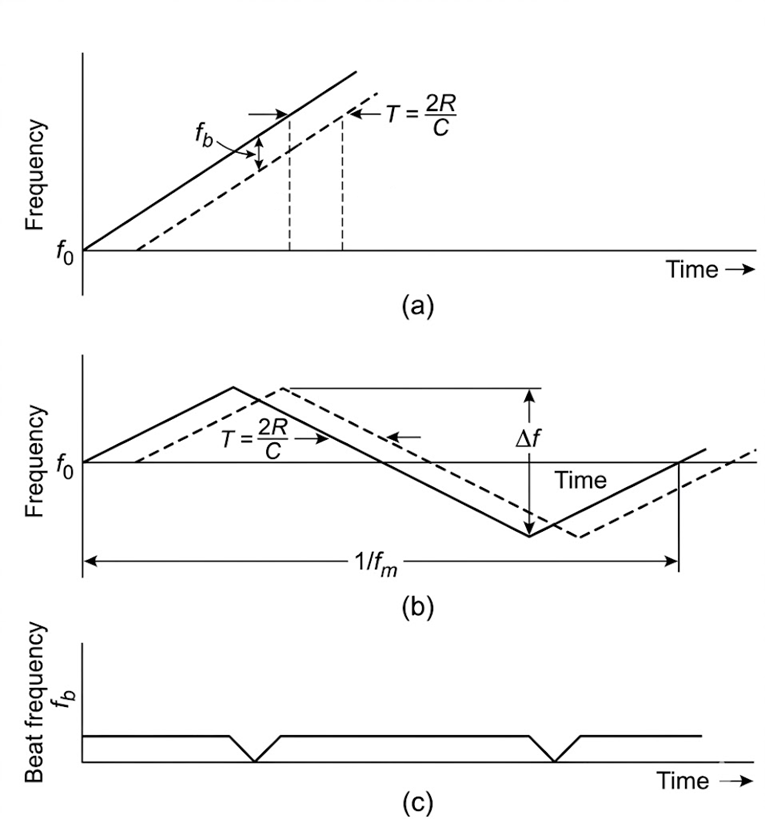
\includegraphics[width=0.75\linewidth]{imagenes/forma de onda - frecuencia modulada.png}
    \caption{Relación frecuencia-tiempo de un radar FMCW. La línea continua representa la señal transmitida y la línea de trazos representa la señal recibida: (a) modulación diente de sierra, (b) modulación triangular y (c) batido de las señales transmitidas y recibidas. (Fuente: \cite{Charvat2014}).}
    \label{fig:fig2.2}
\end{figure}

En el análisis anterior se asumió que el objetivo permanece estacionario. Cuando esta condición no se cumple, el desplazamiento Doppler se superpone a la frecuencia de batido asociada a la distancia, produciendo una variación en la frecuencia resultante. La frecuencia Doppler provoca un desplazamiento vertical en la representación frecuencia-tiempo de la señal reflejada, tal como se muestra en la Figura~\ref{fig:fig2.3}(a). Como consecuencia, durante una parte del ciclo de modulación la frecuencia de batido aumenta debido al efecto Doppler, mientras que durante la otra parte disminuye, tal como se observa en la Figura~\ref{fig:fig2.3}(b).

Por ejemplo, si el objetivo se aproxima al radar, la frecuencia de batido generada durante la rampa ascendente del barrido de frecuencia, denotada por $f_{b,\text{up}}$, resulta igual a la diferencia entre la frecuencia de batido debida al alcance $f_r$ y la frecuencia Doppler $f_D$:

\begin{equation}
    f_{b,\text{up}} = f_r - f_D
\end{equation}

De manera análoga, durante la rampa descendente la frecuencia de batido $f_{b,\text{down}}$ corresponde a la suma de ambas contribuciones:

\begin{equation}
    f_{b,\text{down}} = f_r + f_D
\end{equation}

Estas dos ecuaciones permiten separar los efectos de distancia y velocidad, obteniendo:

\begin{equation}
    f_r = \frac{f_{b,\text{up}} + f_{b,\text{down}}}{2}
\end{equation}

y

\begin{equation}
    f_D = \frac{f_{b,\text{down}} - f_{b,\text{up}}}{2}
\end{equation}

Por lo tanto, mediante el empleo de una modulación triangular de frecuencia es posible estimar simultáneamente la distancia al objetivo y su velocidad radial.

Para determinar el valor de la velocidad radial ($v$) del objetivo, es necesario relacionar la frecuencia Doppler aislada con los parámetros físicos de la onda electromagnética. La relación fundamental del efecto Doppler establece que:

\begin{equation}
    f_D = \frac{2v}{\lambda}
\end{equation}

Donde $\lambda$ representa la longitud de onda de la señal portadora. Despejando la velocidad de esta expresión matemática y sustituyendo la ecuación de la frecuencia Doppler obtenida previamente, el valor final de la velocidad se calcula como:

\begin{equation}
    v = \frac{\lambda}{2} \left( \frac{f_{b,\text{down}} - f_{b,\text{up}}}{2} \right) = \frac{\lambda (f_{b,\text{down}} - f_{b,\text{up}})}{4}
\end{equation}

De esta manera, el procesamiento de las frecuencias de batido en ambas pendientes de la onda triangular proporciona una medición directa de la cinemática del blanco \cite{Charvat2014}.

\begin{figure}[H]
    \centering
    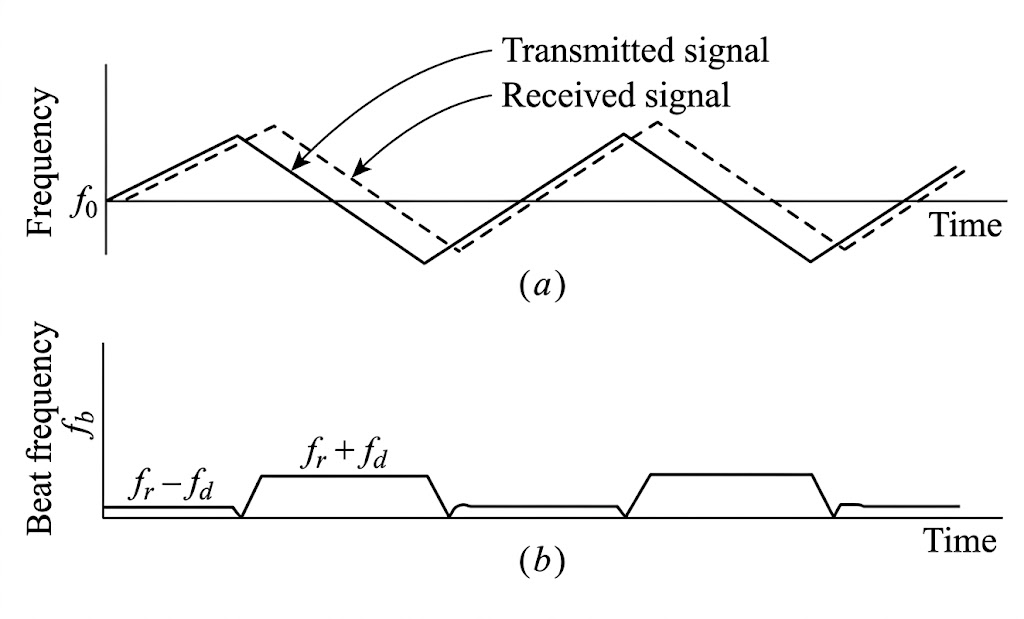
\includegraphics[width=0.75\linewidth]{imagenes/velocidad en onda triangular.png}
    \caption{Relación frecuencia-tiempo con desplazamiento vertical: (a) efecto Doppler y (b) frecuencia de batido. (Fuente: \cite{Charvat2014}).}
    \label{fig:fig2.3}
\end{figure}

\section{Resolución de distancia y velocidad}

\subsection{Resolución de distancia}
La resolución en distancia, o resolución en rango ($\Delta R$), en un radar FMCW define la capacidad del sistema para distinguir de forma individual a dos objetivos que se encuentran espacialmente próximos sobre la misma línea de visión. Si dos blancos están separados por una distancia menor a esta resolución mínima, el radar los detectará como un único objeto en el dominio espectral \cite{skolnik2001}.

En la arquitectura FMCW la resolución espacial teórica depende de forma inversa del ancho de banda del barrido de frecuencia (\textit{chirp}). La expresión matemática fundamental que rige este comportamiento es:

\begin{equation}
    \Delta R = \frac{c}{2B}
    \label{eq:res_rango}
\end{equation}

Donde:
\begin{itemize}
    \item $\Delta R$ es la resolución en distancia [m].
    \item $c$ es la velocidad de propagación de la onda en el vacío ($c \approx 3 \times 10^8\text{ m/s}$).
    \item $B$ es el ancho de banda total de la excursión de frecuencia [Hz].
\end{itemize}

\subsection{Resolución en velocidad}
La resolución en velocidad es la capacidad del radar para distinguir dos blancos que se encuentran a velocidades radiales muy similares.
Dado que la frecuencia Doppler se relaciona con la velocidad radial mediante la ecuación física $f_D = \frac{2v}{\lambda}$, la resolución en velocidad ($\Delta v$) está gobernada por la capacidad del sistema para distinguir mínimas variaciones en $f_D$ \cite{skolnik2001}.

En la modulación triangular, asumiendo que ambas rampas poseen una duración simétrica igual a $T$, el tiempo efectivo de observación para cada medición es $T$. En consecuencia, la resolución frecuencial mínima sobre la que recae el cálculo diferencial es:

\begin{equation}
    \Delta f_{d,\text{min}} = \frac{1}{T}
    \label{eq:res_freq_doppler}
\end{equation}

Igualando esta restricción espectral con la desviación Doppler diferencial inducida por dos objetivos en movimiento relativo ($\Delta f_D = \frac{2\Delta v}{\lambda}$), se obtiene la resolución cinemática base:

\begin{equation}
    \frac{1}{T} = \frac{2\Delta v}{\lambda}
    \label{eq:igualdad_resolucion_vel}
\end{equation}

Despejando analíticamente $\Delta v$, la expresión final para la resolución en velocidad en un sistema de modulación triangular procesado intraciclo es:

\begin{equation}
    \Delta v = \frac{\lambda}{2 T}
    \label{eq:res_velocidad}
\end{equation}

De este desarrollo se evidencia que la capacidad para discriminar velocidades es independiente del ancho de banda de la rampa ($B$).